\chapter{Suppl\texorpdfstring{ementary}{.} material for Chap\texorpdfstring{ter}{.} \getrefnumber{ch:background}}%
\label{ch:SupplBack}

\section{Amino acids}\label{sec:aa}

As shown in \Cref{fig:aaformulas},
the amino acids have different chemical properties.

\begin{figure}[htpb]
    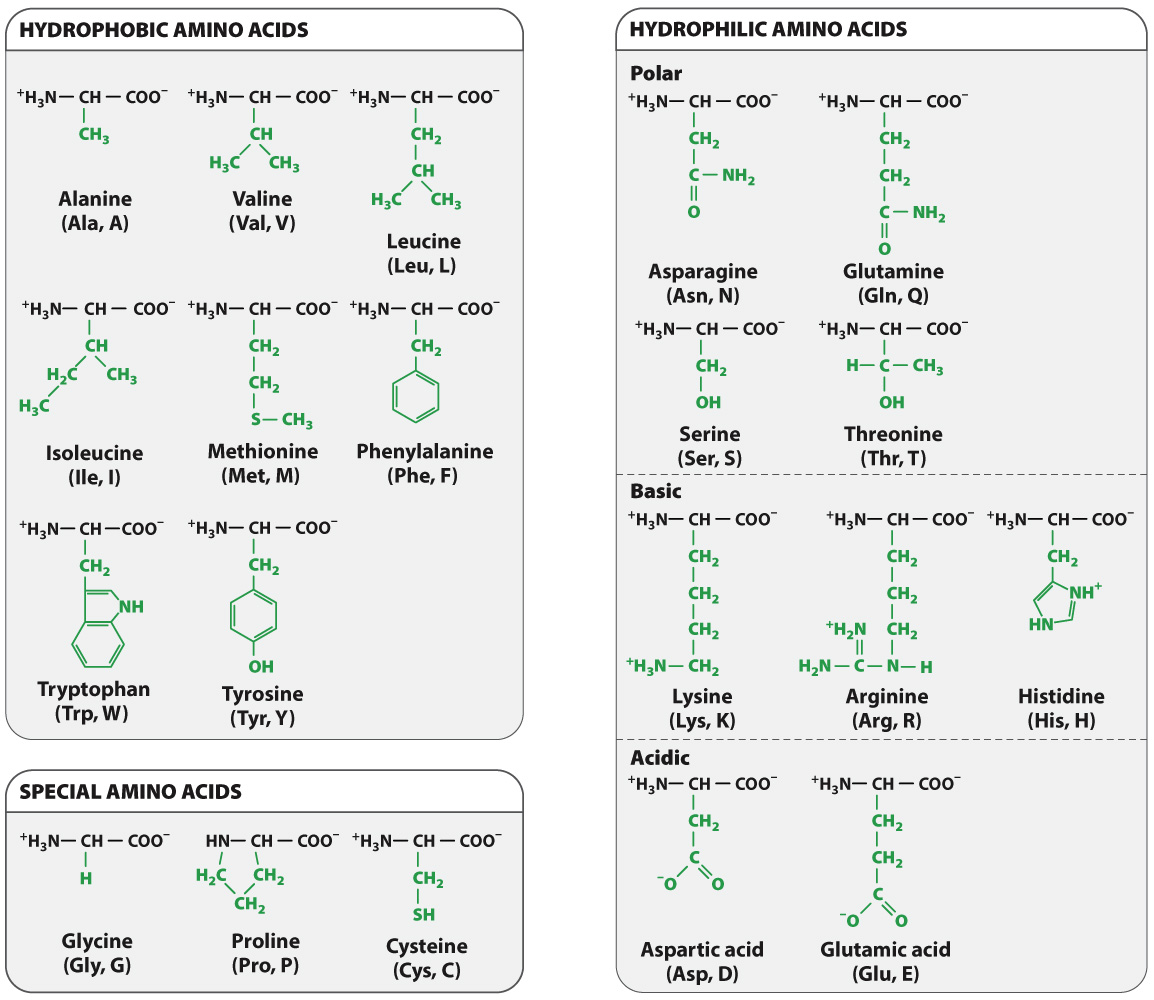
\includegraphics[scale=0.75]{background/aaformulas.jpg}\centering
    \caption[Amino acids formulas]{\label{fig:aaformulas}%
    \textbf{Amino acids formulas} --- from \citet{Morris2016-qv}}
\end{figure}

\section{Original material}\label{sec:kelvinsong}
\vspace{-5mm}
To create \Cref{fig:transcriptionTranslation},
I used original material
by Kelvinsong (\href{https://commons.wikimedia.org/wiki/User:Kelvinsong}{https://commons.wikimedia.org/wiki/User:Kelvinsong}):
\enquote{Simplified diagram of mRNA synthesis and processing. Enzymes not shown.}
(\href{https://commons.wikimedia.org/wiki/File:MRNA.svg}{https://commons.wikimedia.org/wiki/File:MRNA.svg})
and
\enquote{Protein synthesis} (\href{https://commons.wikimedia.org/wiki/File:Protein\_synthesis.svg}%
{https://commons.wikimedia.org/wiki/File:Protein\_synthesis.svg}).

\vspace{-3mm}
\section[EST-sequencing]{Expressed~Sequence~Tag~(EST)~sequencing}\label{sec:EST}
\vspace{-5mm}
\glspl{EST} are short nucleotide sequence generated
from randomly selected \gls{RNA} transcript~\mycite{Parkinson2009-pj}.
\mRNAs\ are reverse transcribed into double-stranded \glspl{cDNA}
(either from the 5' or 3' end of the transcript)~\mycite{Lowe2017-kj}.
These \glspl{cDNA} are cloned to create libraries~\mycite{Harbers2008-qh}
and then sequenced either by Sanger method~\mycite{Sanger1975-io} or
a more high-throughput one such as
the sequencing-by-synthesis (\Cref{subsub:sequencing}).
Although this technique is subject to sampling bias~\mycite{EST} and
often account for only 60\% of an organism expressed genes~\mycite{Bonaldo1996-lx},
it remains a relatively low cost alternative approach to study the transcriptome
(gene discovery).


\vspace{-3mm}
\section{Microarrays}\label{sec:microarray}
\vspace{-5mm}
Microarrays require prior knowledge
(\eg\ annotated genome or \glspl{EST} libraries)
of the organism of interest
as they exploit it to design \emph{probes} (short nucleotide oligomers)
that are arrayed on a solid support (\eg\ glass, silicon thin film cell)%
~\mycite{Lowe2017-kj,Schena1995-tg,Bumgarner2013-ey}.
For transcriptome profiling,
the expressed \glspl{RNA} are first reverse transcribed into \glspl{cDNA}
(also referred as \emph{targets})
and then, after being fluorescently labelled, they are complimentary hybridised
to the microarray probes;
the relative abundance of the transcripts is assessed
by measuring the intensity of the fluorescence
after the excess of unhybridised \glspl{cDNA} is washed away~\mycite{Lowe2017-kj}.
This technology is extremely powerful and popular
as it allows global and parallel analyses of cellular activity.
Microarray technology has also many variations~\mycite{Hoheisel2006-lw}
in addition to its original \gls{cDNA} version
for transcriptional profiling~\mycite{Schena1995-tg}, \eg\
for genotyping~\mycite{Wang1998-rs,Gunderson2006-pp},
protein profiling~\mycite{Hall2007-gt,Sutandy2013-tj,Duarte2017-ao},
splice-variant analysis~\mycite{Cuperlovic-Culf2006-rg} or
transcription factor binding~\mycite{Bulyk2002-ii,Bulyk2007-jc} studies.

\clearpage
\section{FASTQ format}\label{sec:fastq-format}

\begin{figure}[!htbp]
\begin{minipage}[adjusting]{\textwidth}
{\small
{\color[rgb]{0.447059,0.678431,0.274510}\verb!@ERR030856.1!}
{\color[rgb]{0.500000,0.500000,0.500000}\verb!HWI-BRUNOP16X_0001:1:1:2669:1073#0!}%
{\color[rgb]{1.000000,0.000000,0.000000}\verb!/1!}\\
\verb!AAAGGATTATGCAGANGTAGGGCGTGTNNNNNNNNNNNNNGGCTGGGGNNNNNNNNNNNNNNNNNNATNNNCTGACCANCTGAAGTATGTCANGCTGCCT!\\
{\color[rgb]{0.698039,0.145098,0.450980}+}\\
{\color[rgb]{0.000000,0.000000,0.555711}\verb!HHHHHHHIHHFFFFF#>>@>GGGFG###########################################################################!}\\
{\color[rgb]{0.447059,0.678431,0.274510}\verb!@ERR030856.2!}
{\color[rgb]{0.500000,0.500000,0.500000}\verb!HWI-BRUNOP16X_0001:1:1:4476:1072#0!}%
{\color[rgb]{1.000000,0.000000,0.000000}\verb!/1!}\\
\verb!GATAGATTATCAGAANGACAGTTACTTNNNNNNNNNNNNNGGGCACTTNNNNNNNNNNNNNNNNNNATNNNTCATAAGNNCTGTTGCCAAATNAGTGATA!\\
{\color[rgb]{0.698039,0.145098,0.450980}+}\\
{\color[rgb]{0.000000,0.000000,0.555711}\verb!HHHHHHHHHHDDDDD#@@AAGGGGG###########################################################################!}
}
{\footnotesize
Legende:\\
\quad{\color[rgb]{0.447059,0.678431,0.274510}\textbullet Read identifier}\\
\quad{\color[rgb]{0.500000,0.500000,0.500000}\textbullet Optional information (here flow cell lane:tile number:x:y:z)}\\
\quad{\color[rgb]{1.000000,0.000000,0.000000}\textbullet First member of pair (here) or single-end}\\
\quad\textbullet Nucleotide sequence of the read\\
\quad{\color[rgb]{0.698039,0.145098,0.450980}\textbullet Separator (+ or any string of character)}\\
\quad{\color[rgb]{0.000000,0.000000,0.555711}\textbullet Phred score (here Phred 33)}
}
\end{minipage}
\caption{FASTQ format}\label{fig:fastqFormat}
\end{figure}

\FloatBarrier

\section{Phred score}\label{sec:PhredScore}

\begin{table}[!htbp]
\centering
\caption{Phred quality score to accuracy significance}%
\label{PhredtoAccuracy}
\begin{tabular}{@{}lll@{}}
\toprule
\begin{tabular}[c]{@{}l@{}}Phred quality\\ score ($Q$)\end{tabular} & \begin{tabular}[c]{@{}l@{}}Probability of\\ incorrect\\ base call\end{tabular} & \begin{tabular}[c]{@{}l@{}}Base call\\ accuracy\end{tabular} \\ \midrule
10 & 1 in 10 & 90\% \\
20 & 1 in 100 & 99\% \\
30 & 1 in 1,000 & 99.9\% \\
40 & 1 in 10,000 & 99.99\% \\ \bottomrule
\end{tabular}
\end{table}

The \gls{Phred} quality score can be encoded in several standards as shown in \Cref{phredformat}.
%https://en.wikipedia.org/wiki/FASTQ_format#Encoding
\begin{figure}[htbp]
\begin{minipage}[adjusting]{\textwidth}
\begin{verbatim}
SSSSSSSSSSSSSSSSSSSSSSSSSSSSSSSSSSSSSSSSS.....................................................
..........................XXXXXXXXXXXXXXXXXXXXXXXXXXXXXXXXXXXXXXXXXXXXXX......................
...............................IIIIIIIIIIIIIIIIIIIIIIIIIIIIIIIIIIIIIIIII......................
.................................JJJJJJJJJJJJJJJJJJJJJJJJJJJJJJJJJJJJJJJ......................
LLLLLLLLLLLLLLLLLLLLLLLLLLLLLLLLLLLLLLLLLL....................................................
!"#\$\%&'()*+,-./0123456789:;<=>?@ABCDEFGHIJKLMNOPQRSTUVWXYZ[\]^_`abcdefghijklmnopqrstuvwxyz{|}~
 |                         |    |        |                              |                     |
33                        59   64       73                            104                   126
 0........................26...31.......40
                          -5....0........9.............................40
                                0........9.............................40
                                   3.....9.............................40
 0........................26...31........41

S - Sanger        Phred+33, raw reads scores between  0 and 40
X - Solexa        Phred+64, raw reads scores between -5 and 40
I - Illumina 1.3+ Phred+64, raw reads scores between  0 and 40
J - Illumina 1.5+ Phred+64, raw reads scores between  3 and 40
        with 0=unused, 1=unused, 2=Read segment Quality Control Indicator
L - Illumina 1.8+ Phred+33, raw reads scores between  0 and 41
\end{verbatim}
\end{minipage}
\caption{The available Phred score quality score encoding formats}\label{phredformat}
\end{figure}

\begin{figure}[!htbp]
    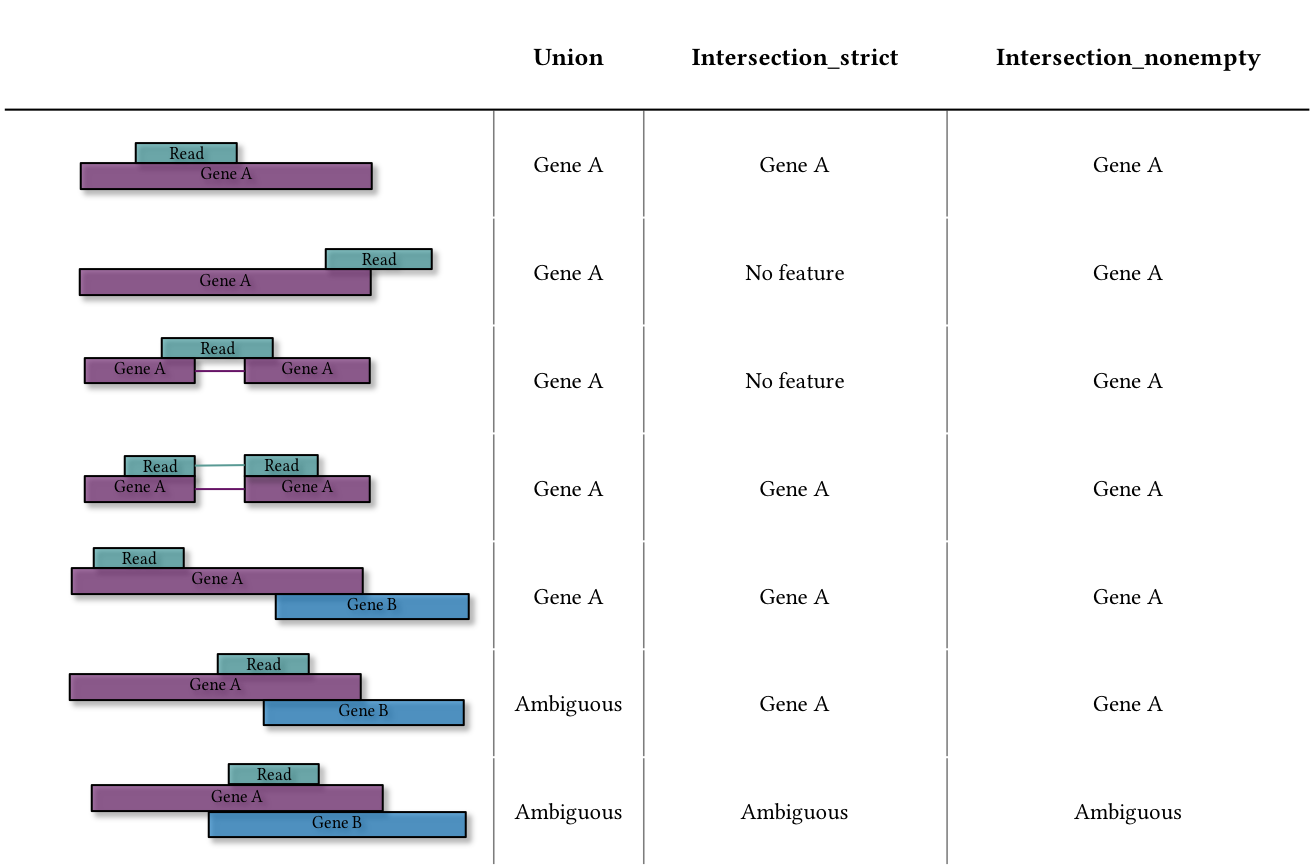
\includegraphics[scale=0.60]{background/interestHtseq}\centering
    \caption[Overlap resolution effects for each \htseq\
    mode]{\label{fig:htseqMode}\textbf{Overlap resolution effects for each \htseq\
    mode.} Each mode resolves a number of overlap situations differently. The
    mode used in this thesis is the \texttt{intersection non-empty} mode. This
    specific mode resolves more situations than the two others. Hence, the loss
    of ambiguous reads is lesser in this mode. [Adaptated from HTseq
    documentation: \footnotesize{\href{http://www-huber.embl.de/HTSeq/doc/count.html}%
    {http://www-huber.embl.de/HTSeq/doc/count.html}}]}
\end{figure}


\begin{table}[]
\centering
\caption{\gls{FPKM} are unsuitable for differential expression analysis}
\label{tab:noFPKM4DEA}
\begin{tabular}{@{}lcccc@{}}
\toprule
\multicolumn{1}{l|}{} & \multicolumn{2}{c|}{Sample 1} & \multicolumn{2}{c}{Sample 2} \\ \midrule
\multicolumn{1}{l|}{} & \multicolumn{1}{c|}{raw counts} & \multicolumn{1}{c|}{normalised counts} & \multicolumn{1}{c|}{raw counts} & normalised counts \\ \midrule
\multicolumn{1}{l|}{$Gene_{1}$} & \multicolumn{1}{c|}{100} & \multicolumn{1}{c|}{0.010} & \multicolumn{1}{c|}{80} & 0.008 \\
\multicolumn{1}{l|}{$Gene_{2}$} & \multicolumn{1}{c|}{100} & \multicolumn{1}{c|}{0.010} & \multicolumn{1}{c|}{80} & 0.008 \\
\multicolumn{1}{c}{\ldots} & \ldots & \ldots & \ldots & \ldots \\
\multicolumn{1}{l|}{$Gene_{i}$} & \multicolumn{1}{c|}{100} & \multicolumn{1}{c|}{0.010} & \multicolumn{1}{c|}{80} & 0.008 \\
\multicolumn{1}{l|}{$Gene_{i+1}$} & \multicolumn{1}{c|}{0} & \multicolumn{1}{c|}{0} & \multicolumn{1}{c|}{2000} & 0.2 \\ \midrule
\begin{tabular}[c]{@{}l@{}}Total number\\ of fragments ($F$)\end{tabular} & 10,000 & 1 & 10,000 & 1 \\ \bottomrule
\end{tabular}
\end{table}

\FloatBarrier

\section{Isotopes of common elements and their natural
frequency}\label{app:isotopes}
\Cref{tab:isotope} lists the mass~\mycite{Audi1993-qn,Audi1995-uk}
and the percent natural abundance~\mycite{Rosman1998-xu}
for stable nuclides (\ie\ atom distinctly characterised by its number of protons (Z)
and number of neutrons (N)) that may be found in \glspl{DNA}, \glspl{RNA} and proteins.

\begin{table}[!htbp]
\centering
\caption[Most common elements and their stable isotopes]%
{\textbf{Most common constitutive elements and their stable isotopes\\ found in DNAs,
RNAs and proteins.} Asterisks (*) mark abundances that are not available.}
\label{tab:isotope}
\begin{tabular}{@{}clccr@{}}
\toprule
\begin{tabular}[c]{@{}c@{}}%
    z \\ (Atomic number)\end{tabular} &
    \multicolumn{1}{c}{Name} & Isotope &
    \begin{tabular}[c]{@{}c@{}}Mass atomic\\ (u)\end{tabular} &
        \multicolumn{1}{c}{\begin{tabular}[c]{@{}c@{}}Natural frequency\\ (\%)\end{tabular}} \\
\midrule
1  & Hydrogen & \isotope[1]{H} & 1.007825 & 99.9885 \\
   & Deuterium & \isotope[2]{H} & 2.014102 & 0.0115 \\
   & Tritium & \isotope[3]{H} & 3.016049 & * \\
6  & Carbon & \isotope[12]{C} & 12.000000 & 98.93 \\
   &  & \isotope[13]{C} & 13.003355 & 1.07 \\
   &  & \isotope[14]{C} & 14.003242 & * \\
7  & Nitrogen & \isotope[14]{N} & 14.003074 & 99.632 \\
   &  & \isotope[15]{N} & 15.000109 & 0.368 \\
8  & Oxygen & \isotope[16]{0} & 15.994915 & 99.757 \\
   &  & \isotope[17]{0} & 16.999132 & 0.038 \\
   &  & \isotope[18]{0} & 17.999160 & 0.205 \\
15 & Phosphorus & \isotope[31]{P} & 30.973762 & 100 \\
16 & Sulphur & \isotope[32]{S} & 31.972071 & 94.93 \\
   &  & \isotope[33]{S} & 32.971458 & 0.76 \\
   &  & \isotope[34]{S} & 33.967867 & 4.29 \\
   &  & \isotope[35]{S} & 35.967081 & 0.02 \\
53 & Iodine & \isotope[127]{I} & 126.904468 & 100 \\
\bottomrule
\end{tabular}
\end{table}

